\begin{frame}{Generate Knowledge Prompting}
  \vspace{-0.5em}
  \begin{itemize}
    \item This technique involves using additional knowledge provided as part of the context to improve results on complex tasks such as commonsense reasoning
    \item The knowledge used in the context is generated by a model and used in the prompt to make a prediction
    \begin{itemize}
      \item Highest-confidence prediction is used
    \end{itemize}
  \end{itemize}
  \vspace{0.2em}
  \begin{center}
    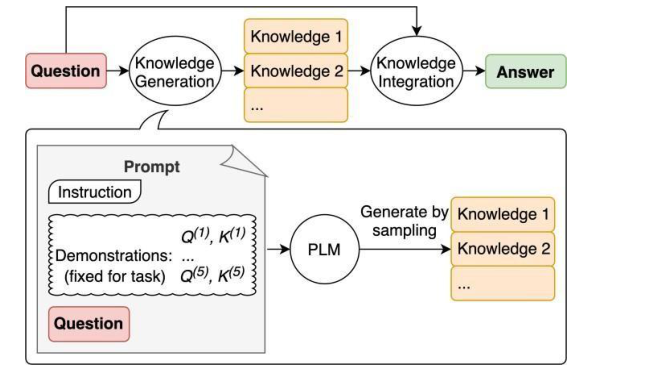
\includegraphics[width=0.75\textwidth, height=0.48\textheight, keepaspectratio]{images/prompting-rag/prompting_knowledge_generation_pipeline.png}
  \end{center}
  \vspace{0.1em}
  {\scriptsize
    \color{gray!75!black}
    Source: Liu et al., ACL 2022, \url{https://arxiv.org/abs/2110.08387}
  }
\end{frame}

\begin{frame}{Generate Knowledge Prompting Example}
  \vspace{-0.7em}
  \begin{itemize}
    \item The first step is to generate knowledge. Below is an example of how to generate the knowledge samples:
  \end{itemize}
  \vspace{0.3em}
  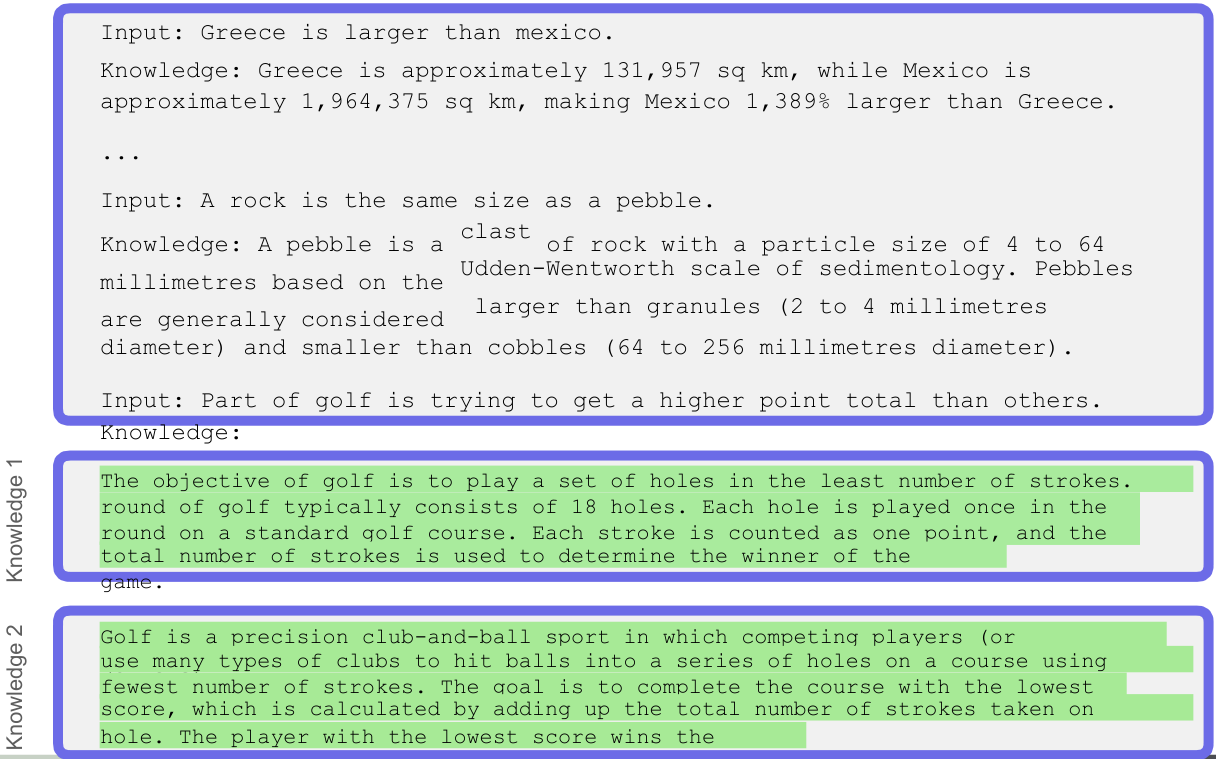
\includegraphics[width=0.77\textwidth, height=0.65\textheight, keepaspectratio]{images/prompting-rag/prompting_knowledge_generation_examples.png}

  {\scriptsize
    \color{gray!75!black}
    Source: DAIR.AI Prompt Engineering Guide, \url{https://www.promptingguide.ai/techniques/knowledge}
  }
\end{frame}

\begin{frame}{\strut\hspace{-0.25em}Generate Knowledge Prompting Example}
  \vspace{-1em}
  \begin{itemize}
    \item The knowledge samples are then used to generate \textbf{knowledge augmented questions} to get answer proposals.
    \item The highest-confidence response is selected as final answer.
  \end{itemize}
  \vspace{0.1em}
    \begin{center}
      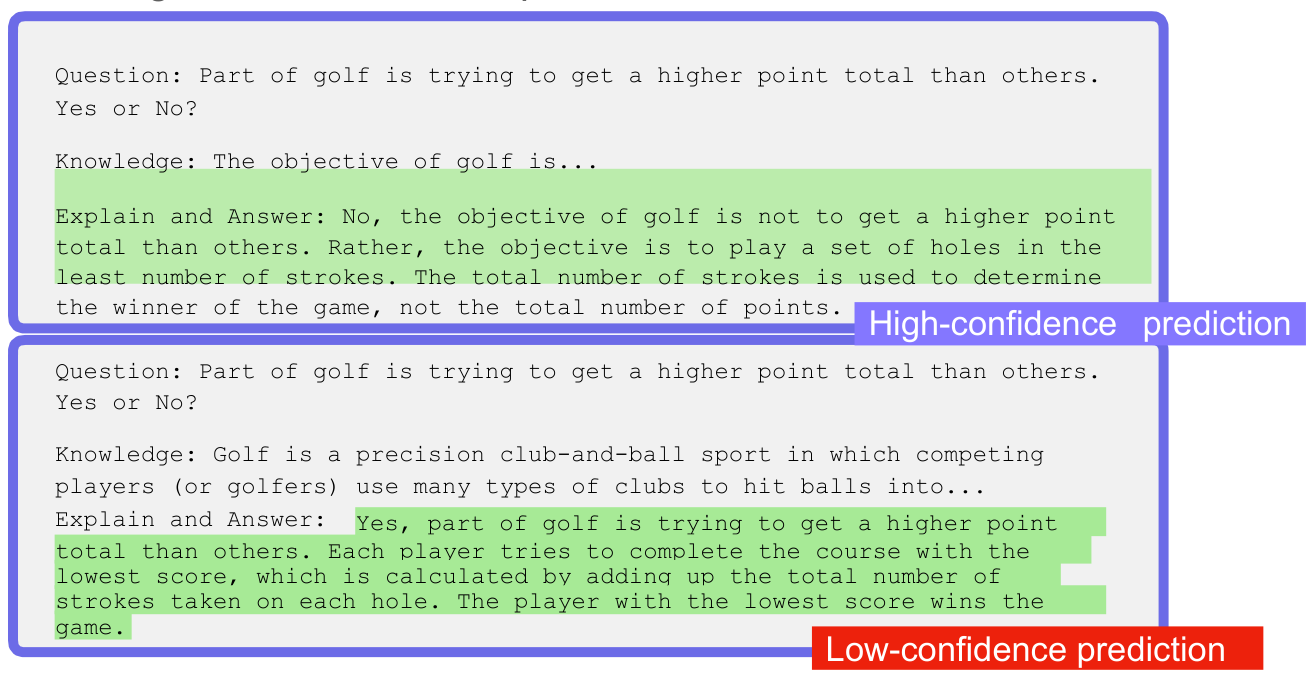
\includegraphics[width=0.77\textwidth, height=0.62\textheight, keepaspectratio]{images/prompting-rag/prompting_knowledge_confidence_predictions.png}
    \end{center}
  \vspace{-0.5em}
  {\scriptsize
    \color{gray!75!black}
    Source: DAIR.AI Prompt Engineering Guide, \url{https://www.promptingguide.ai/techniques/knowledge}
  }
\end{frame}

\begin{frame}[t]{Program-aided Language Model (PAL)}
  \begin{itemize}
    \item Chain-of-thought prompting is a good example of how to steer models to perform better at complex reasoning tasks
    \begin{itemize}
      \item[] \begin{minipage}[t]{0.85\textwidth}
        \small However, sometimes CoT is not enough as it depends only on the generated text from the model
      \end{minipage}
    \end{itemize}
    \vspace{0.5em}
    \item Program-aided language models (PAL) use an LLM to read problems and generate programs as the intermediate reasoning steps
    \begin{itemize}
      \item[] \begin{minipage}[t]{0.85\textwidth}
        \small It offloads the solution step to a runtime such as Python interpreter
      \end{minipage}
    \end{itemize}
  \end{itemize}
  \vfill
  {\scriptsize
    \color{gray!75!black}
    Source: Gao et al., ``PAL: Program-aided Language Models'', ICML 2023, \url{https://arxiv.org/abs/2211.10435}
  }
\end{frame}

\begin{frame}{Program-aided Language Model (PAL) Example}
  \centering
  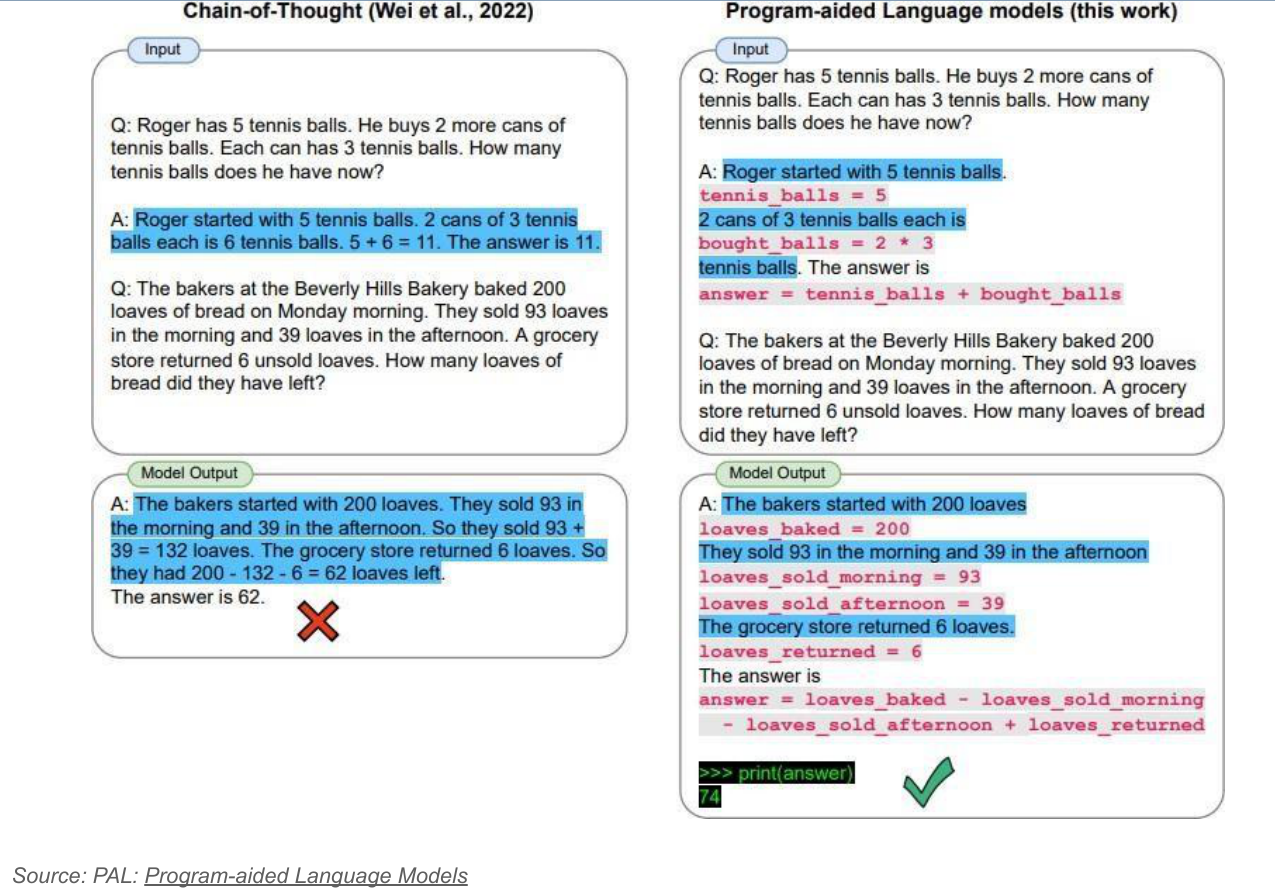
\includegraphics[width=0.9\textwidth, height=0.82\textheight, keepaspectratio]{images/prompting-rag/prompting_program_aided_lm_comparison.png}

  {\scriptsize
    \color{gray!75!black}
    Source: Gao et al., ICML 2023, \url{https://arxiv.org/abs/2211.10435}
  }
\end{frame}
